\chapter{System Demands, Comparisons and Decisions}
\label{chptr:redundantSystemsCompare}
Due to high demands on the safety and reliability of an on-board unit, it is to be developed as a redundant system.
As previously described, there are different approaches and concepts to redundancy.
In order to evaluate the reliability of different redundant architectures and concepts, the developed system's functional requirements need to be known.
Furthermore, possible security risks and catastrophic failures must be known in order to be able to come up with a suitable system architecture.
\\

\noindent
In the first section of this chapter, an \abr{ETCS} on-board system's demands are described.
For this purpose, an \abr{ETCS} scenario - which is derived from the \abr{ETCS} specification - is presented.
Based on this scenario, further investigations are made.
Afterward, a fault model is established and \abr{DDS} building blocks are introduced that lay the foundation for the following comparison of redundant architectures.
Then, based on \abr{TMR}, different redundancy architectures are developed and evaluated.
Finally, the system comparison is summarized and a final system architecture, as well as a synchronization model, are presented.

\section{System Demands}
As already stated, the system that is developed in this thesis is intended to function as an on-board unit within \abr{ETCS} level two.
As such, it receives information from the \abr{RBC}, estimates the train's position based on sensor data, observes the train's braking curve, and evaluates telegrams from track-side balises.
For demonstration purposes, a subset of \abr{ETCS} level two is considered.
In the following, the \abr{ETCS} subset as well as the resulting system requirements are described.

\subsection{Scenario Description}
\label{sec:ScenarioDescription}

The considered on-board system should process \abr{ETCS} scenarios.
Such a scenario consists of a \abr{MA}, a set of linked balises, and track-side balises.
In each scenario, the train goes through a journey that begins as soon as the train starts moving and stops when it brakes.
\\

\noindent
As such, the system should be able to receive a \abr{MA} that contains driving permissions.
Therefore, each \abr{MA} consists of a start- and an end position that limit an area where the train is authorized to move.
Furthermore, the system should be able to receive a list of balises that the train will encounter during its journey.
The balises in this list have a position and an unique identifier.
The phase in which the balise positions and identifiers are sent and received is called \textit{linking phase}.
Further, the tuples of balise position and identifier that are transmitted during the linking phase are called \textit{linked balises}.
Upon receiving a \abr{MA} and a list of linked balises the train starts its journey.
While driving, the on-board unit evaluates sensor data and calculates the train's position based on these data and the \abr{MA}'s starting position.
Due to possible inaccuracies, a confidence interval for the train's position is calculated.
In addition, the on-board unit should be capable of receiving balise telegrams from track-side balises.
Such balise telegrams consist of an unique identifier so that they can be assigned to a linked balise.
When receiving a balise telegram, the train's position is set to the balise's position and the confidence interval is reset.
\\

\noindent
During an entire journey, the train's braking curve needs to be periodically calculated and coordinated with the \abr{MA}'s end position.
Thereby, it is ensured that the train will not drive past the \abr{MA}'s boundaries.

An algorithm for calculating a train's braking curve in \abr{ERTMS} systems is presented by B. Friman~\cite{CalculateBrakeCurveFriman}.
In general, three types of information are considered for supervising a braking curve, namely speed restrictions, track gradients, and a train's characteristic deceleration abilities.
For calculating a train's braking distance $dbr$ for a train with a deceleration ability of $dec$ from one speed $v_1$ to another speed $v_2$, the following equation can be used:

\begin{equation}
dbr = \frac{{v_1}^2}{2*dec} - \frac{{v_2}^2}{2*dec}
\end{equation}

\noindent
The train's speed is measured in $m/s$ and its deceleration ability is measured in $m/s^2$.
For the considered scenario, it is assumed that the track is flat so that the braking curve solely depends on the train's speed and deceleration abilities.
\\

\noindent
The subset is derived from the ETCS specification subset 026~\cite{ETCS26}.
It can be used as a valid subset to show the solution's functionality since it only truncates the information but not the requirements.
For example, the subset used here uses individual balises instead of balise groups.
Thereby, the information on the direction of travel is lost.
However, the safety-related requirements concerning the positioning of the track components are retained.
This allows the findings of a solution that satisfies the subset fault model to be applied to the entirety of \abr{ETCS}.

\subsection{Fault Model}
\label{subsec:faultModel}
The safety requirements for the system are based on the fault classes \textbf{F1}-\textbf{F4} from~\autoref{sec:techniquesSafetyReliability}\cite{CristianFaultModel}.
Consequently, crash faults, omission faults, timing faults, and computation faults need to be considered.
Byzantine faults are not covered.
\\

\noindent
During a train's journey, situations may arise that affect its safety.
The deployed system should be able to detect the following problems:

\begin{enumerate}
\item When the braking curve calculation shows that the train reaches the end of the \abr{MA}.
\item A balise telegram is received whose associated balise is not linked.
\item The balise telegram from a linked balise is received, but the linked position is outside the system's current confidence interval.
\end{enumerate}

\noindent
In the event of one of the problems described above, the system must stop the train.
In a simulation, it is sufficient to generate an appropriate notification.
In practice, the train's brakes need to be controlled for this purpose.
To interface with the brakes, additional hardware that can be controlled by switching currents is required.
\\

\noindent
In the context of this work, problems related to receiving and processing inputs are considered.
The applied components' internal consistency is not monitored.
This means that hardware faults can lead to component failures.
Since the system is operating in a safety-critical environment, individual component failures need to be mitigated to not affect the system's safety.
Therefore, redundancy concepts are applied.

In the redundant system, a voter performs a majority voting and thereby generates a final system decision.
For the voter to perform a vote, individual replica's decisions need to be submitted to the voter.
Therefore, the communication channel and the \abr{DDS} middleware are expected to be safe and reliable.
Hence, it is assumed that no data is lost or corrupted during transmission.

\section{\glsentryfull{DDS} Building Blocks}

Information in \gls*{ETCS} can be diverse in terms of type, size, durability, update frequency, and priority.
For example, a train's position is a periodically and frequently updated type of information, while a \gls*{MA} is valid for a longer time and may be updated infrequently.
There is also a difference between whether the information is kept as a state of the system, used as a message within the system, or provided as system input.
The system's state is typically derived from input events.
In this section, an overview of different information types and possibilities for their representation in \gls*{DDS} topics is provided.

\begin{table}[htbp!]
	\begin{center}
		\caption{\Gls*{QOS} policies for volatile and enduring state topics in a \gls*{DDS} system. For an enduring state, data changes rarely and unperiodically. In volatile states, data changes frequently and periodically. State topics can be used to share a global system state among all participants.}
		\label{tab:stateQOS}
		\begin{tabularx}{\textwidth}{|X|X|X|X|}
			\hline
			\textbf{QoS policy} & \textbf{Setting for volatile state} & \textbf{Setting for enduring state} & \textbf{Description}\\
			\hline \hline
			Deadline & Depends on actual implementation & Not required & For volatile states, the deadline should match the period in which the data updates. \\
			\hline
			DestinationOrder & SourceTimestamp & SourceTimestamp & Order by source timestamp guarantees that always the most recent data is stored. \\
			\hline
			Durability & Volatile & Transient or Persistent & The more frequent the state changes, the less critical it is for late joining subscribers to see previously published data. \\
			\hline
			History & KeepLast(1) & KeepLast(1) & Most of the time, only the last state matters. \\
			\hline
			LatencyBudget & Depends on actual implementation & Not required & The maximum acceptable delay for sending the data should be chosen so that deadlines are not missed. \\
			\hline
			Reliability & BestEffort & Reliable & For rapidly and periodically changing states, it is ok if some data get lost. For enduring state, however, data has to be transferred reliably. \\
			\hline
			WriterDataLifecycle & Not required & Do not dispose unregistered instances & Even if data instances are unregistered, the actual data on enduring state topics should not be disposed. \\
			\hline
		\end{tabularx}
	\end{center}
\end{table}

A train's speed or position data, as well as currently valid \abrpl{MA}, are examples of the system's state.
A state could contain periodically changing data, or irregular changing data, respectively.
A state whose data changes periodically is called a volatile state, while a state whose data changes slow and irregular is called an enduring state.
Possible \gls*{QOS} settings for volatile and enduring states are presented in~\autoref{tab:stateQOS}.

\begin{table}[htbp!]
	\begin{center}
		\caption{\Gls*{QOS} policies for event topics in a \gls*{DDS} system. Event topics can be used to for \abr{RPC} to make inquiries and invoke functionality from other components.}
		\label{tab:eventQOS}
		\begin{tabularx}{\textwidth}{|X|X|X|}
			\hline
			\textbf{QoS policy} & \textbf{Setting} & \textbf{Description}\\
			\hline \hline
			Deadline & Depends on actual implementation & For periodically updating events, a deadline can be specified to detect when events are missing in a period. \\
			\hline
			DestinationOrder & SourceTimestamp & The event samples should be ordered based on the time they got produced. \\
			\hline
			Durability & Depends on actual implementation & It might be appropriate to let late joining DataReaders process the events. \\
			\hline
			History & KeepAll & All events shall eventually be sent and processed. Therefore, the event samples should be stored on both the sender and the receiver side.  \\
			\hline
			Lifespan & Depends on actual implementation & An event may be only valid for a specific period of time. This timespan can be specified by assigning a lifespan to a DataWriter. \\
			\hline
			Reliability & Reliable & The middleware will attempt to deliver all event data samples and actively checks if the receivers got them. In case the samples got lost, they are re-transmitted. \\
			\hline
			ResourceLimits & Depends on actual implementation & It might be appropriate to specify an upper bound for resources to be allocated. Especially with History set to KeepAll. \\
			\hline
			WriterDataLifecycle & Do not dispose unregistered instances & Unregistered data instances should not be disposed because the events are required to be eventually processed. \\
			\hline
		\end{tabularx}
	\end{center}
\end{table}

Certain circumstances, such as the availability of track-side information or the exceeding of speed limits, need to be processed as soon as possible.
Such data is typically expressed as events and can be represented using event topics.
\autoref{tab:eventQOS} provides an overview about \gls*{QOS}-policy settings for event topics.
The presented combination of \abr{QOS}-settings ensures that events are eventually processed in the order they were issued and that no event is omitted.
While some settings are universal for event topics, some others need to be evaluated with regards to actual system implementation and consequential requirements.


\section{Architecture Comparisons}
As proposed by Johnson Barry, the different redundancy techniques are applicable for different use-cases~\cite{BarryFaultToleranceAnalysis}.
In this section, different redundancy techniques are selected, combined, and evaluated based on the following criteria:

\begin{itemize}
\item \textbf{Reliability:} How likely does the system continue to operate as specified in case of faults?
\item \textbf{Safety:} Can system faults lead to catastrophic failures?
\item \textbf{Implementability using \gls*{DDS}:} How easy is it to implement the redundant architecture using \abr{DCPS} concepts?
\end{itemize}

\noindent
In order to evaluate the redundant system's reliability, it is mathematically evaluated using Markov Chains, which were described in~\autoref{sec:techniquesSafetyReliability}.
To assess the system's safety, situations where faults can lead to catastrophic failures are assessed. 
For investigating the technique's implementability with \gls*{DDS}, possible \abr{DDS} building blocks for communication and state are examined.
\\

\noindent
Regardless of the specific architecture, the system should receive and process inputs via a \abr{DDS} event topic.
For specific inputs - in this work balise telegrams - an output in form of a decision should be generated.
In order for the system to generate a single output, the utilized replicas require to communicate with one another via \abr{DDS} event topics.
Further, the replicas should be able to access a global system state managed via \abr{DDS} state topics to make deterministic decisions.
Other design decisions are architecture-specific.
\\

\noindent
In the following, characteristics of different redundant architectures are evaluated.
One of the most commonly used redundancy techniques is \abr{TMR}~\cite{FaultToleranceViaNMR}, which will therefore constitute the foundation for further system investigations.

\subsection{\glsentryfull{TMR}}
The minimal communication overhead required in \abr{TMR} is between the replicas and the voter.
As described earlier, voters can either be implemented in software or hardware.
This does not hold for redundant systems where \gls*{DDS} is used for the communication between the replicas and the voter because the voter always requires a software part that implements the \gls*{DCPS} standard.
Specialized hardware that implements the \abr{DCPS} standard would be too expensive.
\\

\noindent
\Gls*{TMR} has already been briefly discussed in~\autoref{sec:redundancyPatterns} and is depicted in~\autoref{fig:Classical2OO3}.
The reliability and safety characteristics of \gls*{TMR} have been studied in depth, for example by Arifeen \etal~\cite{ArifeenFaultTolerantTMR}.
Their findings show that the reliability of \gls*{TMR}-systems ($R_{TMR}(t)$) is given by the sum of the probability of all three components functioning and two components functioning as specified.

\begin{equation}
R_{TMR}(t) = 3e^{-2 \lambda t} - 2e^{-3 \lambda t}
\end{equation}

\noindent
This equation only holds for homogeneous redundancy and when the components are independent.
While the independence is a precondition for the exponential failure law, a diverse system can be described in the same way by using a distinct $\lambda$ for each component.
\\

\noindent
The first four fault classes from~\autoref{sec:techniquesSafetyReliability} for at most one failing replica can be tolerated by a \abr{TMR} system.
For example, if one replica produces a wrong result, the voter still receives two correct results and can mask the wrong result using a majority voting.
However, if two or more replicas produce the same - but wrong - result, the voter erroneously accepts the wrong result as the majority.
On the other hand, if two or more replicas fail to produce on output within a certain time span, the voter can detect this as a deadline violation and transfer the system into a safe state, e.g. by stopping the train.
Therefore, only \textbf{F1}, \textbf{F2}, and \textbf{F3} can be detected when more than one replica is affected in \abr{TMR}.

In order to allow more than one component to generate a wrong result without affecting the system's safety, component checking mechanisms could be applied using the concepts of~\cite{DistributedSafety2020}.
Thereby, a wrong result can be identified as being wrong and excluded from the voting process.
\\

\noindent
Nevertheless, a failed voter can render the entire system unsafe because it marks a single point of failure in \abr{TMR}.
Therefore, the entire system's reliability and safety cannot be higher than the voter's reliability and safety~\cite{ArifeenFaultTolerantTMR}.

Another problem arises when the frequency in which inputs occur is higher than the time that the system needs to produce an output.
In such a case, an output might be already outdated even before it is being produced.
\\

\noindent
Recapped, \abr{TMR} bears three significant challenges, which are:

\newcommand{\ChallengeWR}{\textbf{Multiple Wrong Results}\xspace}
\newcommand{\ChallengeVoter}{\textbf{Single Voter}\xspace}
\newcommand{\ChallengeThrough}{\textbf{Throughput Cap}\xspace}
\begin{itemize}
\item \ChallengeVoter The voter marks a single point of failure.
\item \ChallengeWR The system's safety is compromised when more than one replica produces a wrong result.
\item \ChallengeThrough When inputs occur in a higher frequency than the system's throughput time, delays happen that can compromise the system's safety.
\end{itemize}

\noindent
In order to solve \ChallengeVoter and prevent the voter from being a single point of failure, redundancy can be introduced for the voters as well.
However, this introduces new challenges such as the possibility of a split-brain, where multiple voters are active and can manipulate the output simultaneously.
\\

\noindent
In order to overcome the \ChallengeWR challenge, additional replicas can be added to the system.
It can be shown via induction that adding more replicas increases a system's reliability.

\begin{itemize}
\item \emph{Proof by Induction}: Let $M$ be constant and $M \leq N$, let $R_{c}$ be the reliability of the system's components.
\begin{itemize}[label=$\lozenge$, itemsep=2ex]
\item \emph{Base Case:}
\begin{align*}
&\text{Let}~N = 1 \Rightarrow M = 1.\\
&R_{1oo1} = {1 \choose 1} * R_{c}^1 * (1 - R_{c})^0 = R_{c}
\end{align*}

\item \emph{Hypothesis:} $R_{MooN}$ describes the reliability for an M-out-of-N-system and a components reliability $R_{c}$ can only be positive.

\item \emph{Induction Step(s):}
\begin{align*}
R_{MooN+1} &= \sum_{i=M}^{N+1} {N + 1 \choose i} * R_{c}^i * (1 - R_c)^{N + 1 - i}\\
&= \sum_{i=M}^{N} {N \choose i} * R_{c}^i * (1 - R_c)^{N - i} + {N+1 \choose N+1} * R_c^{N+1} * (1 - R_c)^{N+1 - N+1}\\
&= R_{MooN} + R_c^{N+1} \\
&\Rightarrow R{MooN} \leq R_{MooN+1} \quad \square
\end{align*}
\end{itemize}
\end{itemize}

\noindent
Additional components can be added in an active and in a passive hardware redundant way.
Adding a spare replica is a possibility to address the \ChallengeWR problem.

\subsection{\glsentrylong{TMR} with Spares}
\begin{figure}[!ht]
	\centering
	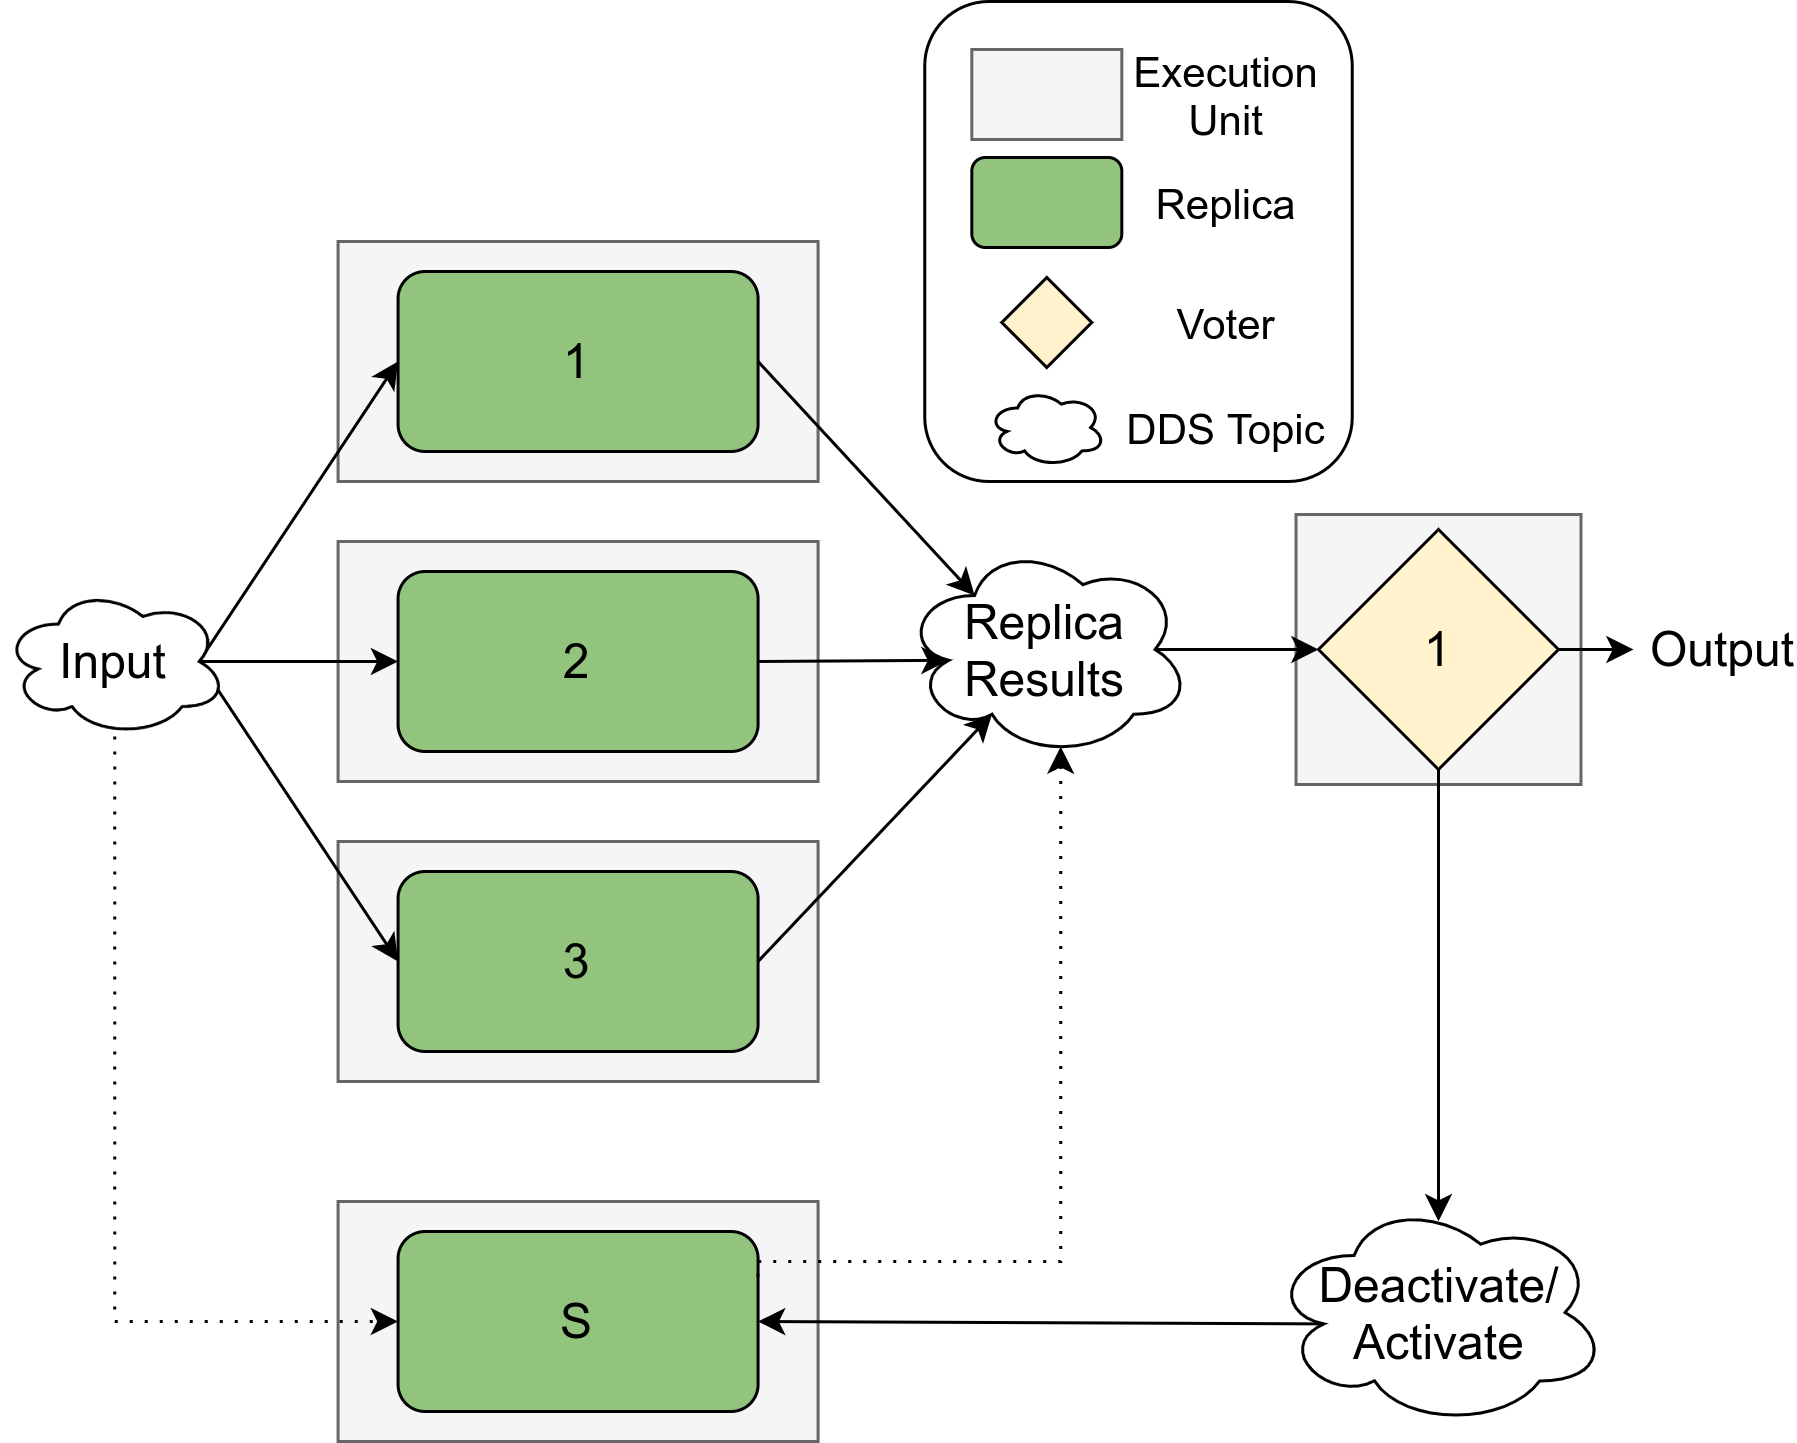
\includegraphics[width=0.8\linewidth]{images/TMRWithSparesDDS}
	\caption{A hot standby can be implemented using a \abr{DDS} event topic to send \textit{activate} and \textit{deactivate} events. The voter unit is responsible for detecting a failed replica and thereupon activates the spare component (S) by sending a corresponding event.}
	\label{fig:TMRWithSparesDDS}
\end{figure}

Instead of adding more replicas in a passive hardware redundancy way, they can also be added as spares in an active hardware redundancy approach.
However, this also increases costs and communication overhead.

Standby redundancy is a way for redundant systems to repair themselves in case of failures by adding spare replicas that can replace faulty replicas.
Therefore, the system relies on error detection methods.
For the reliability of \abr{TMR} systems with one spare component holds - provided that the system can reliable detect and repair any error and the replicas are homogeneous and independent:

\begin{equation}
R_{TMR\_S}(t) = 2 * {3 \choose 3} e^{-\lambda t} + {3 \choose 2} e^{-\lambda t}
 = 3e^{-2 \lambda t} - e^{-3 \lambda t}
\end{equation}

\noindent
One way of implementing \abr{TMR} with a spare using \abr{DDS} is depicted in~\autoref{fig:TMRWithSparesDDS}.
The input, as well as the replica's results and an activate event, are modeled as \abr{DDS} event topics.
In an exemplary case where one replica crashes, the voter receives only two replica results and thereupon sends an \textit{activate} event via the corresponding topic.
When the spare replica \textbf{(S)} receives the activate event, it subscribes to the \texttt{Input} topic and registers to the \texttt{Replica Results} topic to publish data to it.
If the failed replica comes back to life and the voter recognizes this, the voter can reject the result from \textbf{(S)} and send a \textit{deactivate} event.
After that, the spare replica ends its subscription to the input topic and stops publishing results.
A precondition for this approach is that a replica's result can be unambiguously assigned to a replica, for example by using IDs or by using an individual result topic for each replica.
Further, the spare replica's state needs to be synchronized with the other replicas to make pertinent decisions, which can be assured by managing a global system state through \abr{DDS}.
\\

\noindent
Although \abr{TMR} with spares improves the replicated system's reliability and safety by allowing more replicas to fail (\ChallengeWR), the voter remains a single point of failure (\ChallengeVoter) and the system's throughput has not changed (\ChallengeThrough).
An often applied technique for improving a system's throughput is pipelined computation~\cite{TanenbaumSteen07}.
Hence, a pipelined \abr{TMR} approach is considered in the following.

\subsection{Pipelined \glsentrylong{TMR}}
\begin{figure}[!ht]
	\centering
	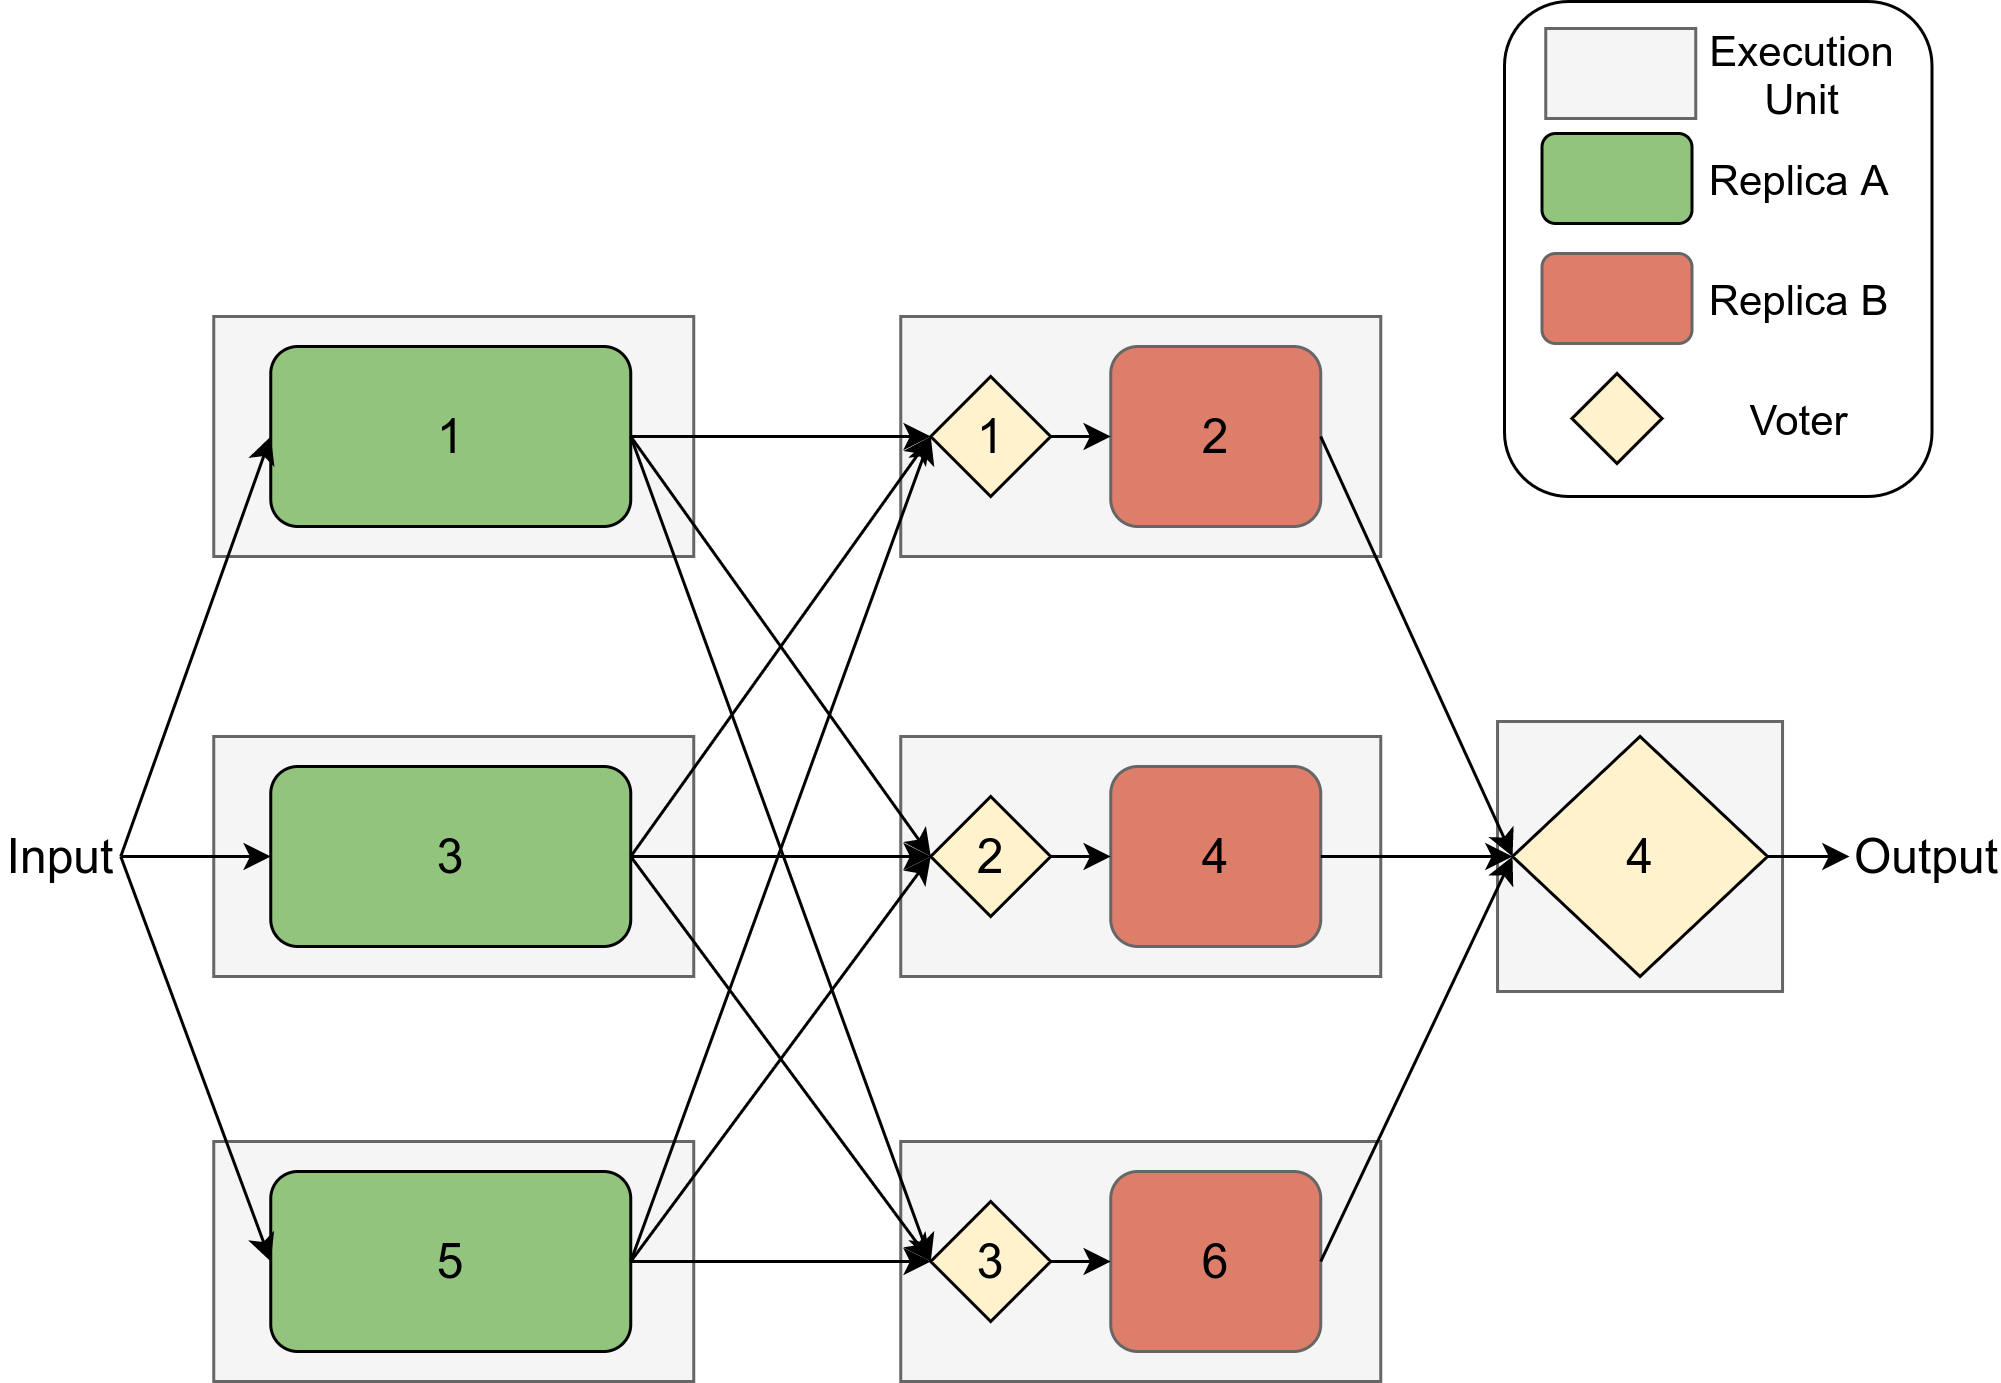
\includegraphics[width=0.9\linewidth]{images/InterconnectedVoterPipeline}
	\caption{A \abr{TMR} architecture with interconnected pipelines can increase the system's throughput and facilitate intermediate voting to reduce provisional result's effect on the final output. In this example, replicas of type \textbf{B} perform voting on the results of type \textbf{A} replicas before further processing. Thus, type \textbf{B} replicas mask a failure of a type \textbf{A} replica before it can affect the final output.}
	\label{fig:PipelineIntermediateVoters}
\end{figure}

In a pipelined approach, intermediate voting should be used to reduce the effects of wrong intermediate results.
It is further possible that components function as both a voter and a data processing replica.
A redundant and pipelined system with intermediate voting on replicas is depicted in~\autoref{fig:PipelineIntermediateVoters}, where voters \textbf{(1)}, \textbf{(2)}, and \textbf{(3)} each perform a majority voting based on the results from replicas \textbf{(1)}, \textbf{(3)}, and \textbf{(5)}.
Based on the intermediate voter, replicas \textbf{(2)}, \textbf{(4)}, and \textbf{(6)} can perform their dedicated calculations and produce individual outputs, which are later processed by the voter \textbf{(4)}.
Thereby, any failure from replicas \textbf{(1)}, \textbf{(3)}, or \textbf{(5)} can be masked before they are further processed and handled to the final voter \textbf{(4)}.
However, this approach is still a two-out-of-three approach and therefore has the same challenges that \abr{TMR} has.
Further, the pipelined approach's reliability can be calculated in the same way as for \abr{TMR}, because in the worst case, two replicas of type \textbf{A} or type \textbf{B} could fail.
\\

\noindent
Although the pipelined approach enhances the system's throughput, it also enhances the computation and communication overhead, as well as the system's cost.
Thus, a trade-off needs to be made between the added throughput and the additional computation,  as well as the communication overhead and the increased cost for the system.
\\

\noindent
Again, the reliability evaluation can only be made without evaluating the voter - in the pipelined version voter \textbf{(4)} - which remains a single point of failure.
The voter can be prevented from being the single point of failure by adding redundancy for the voter as well, like for voters \textbf{(1)}, \textbf{(2)}, and \textbf{(3)} in~\autoref{fig:PipelineIntermediateVoters}.
In such a system, it needs to be ensured that only a single voter is in charge of controlling the system's final output.
This can be achieved by applying a consensus algorithm.

\subsection{Consensus-inspired Architectures}
\label{subsec:consensusArchitecture}
\begin{figure}[!h]
	\centering
	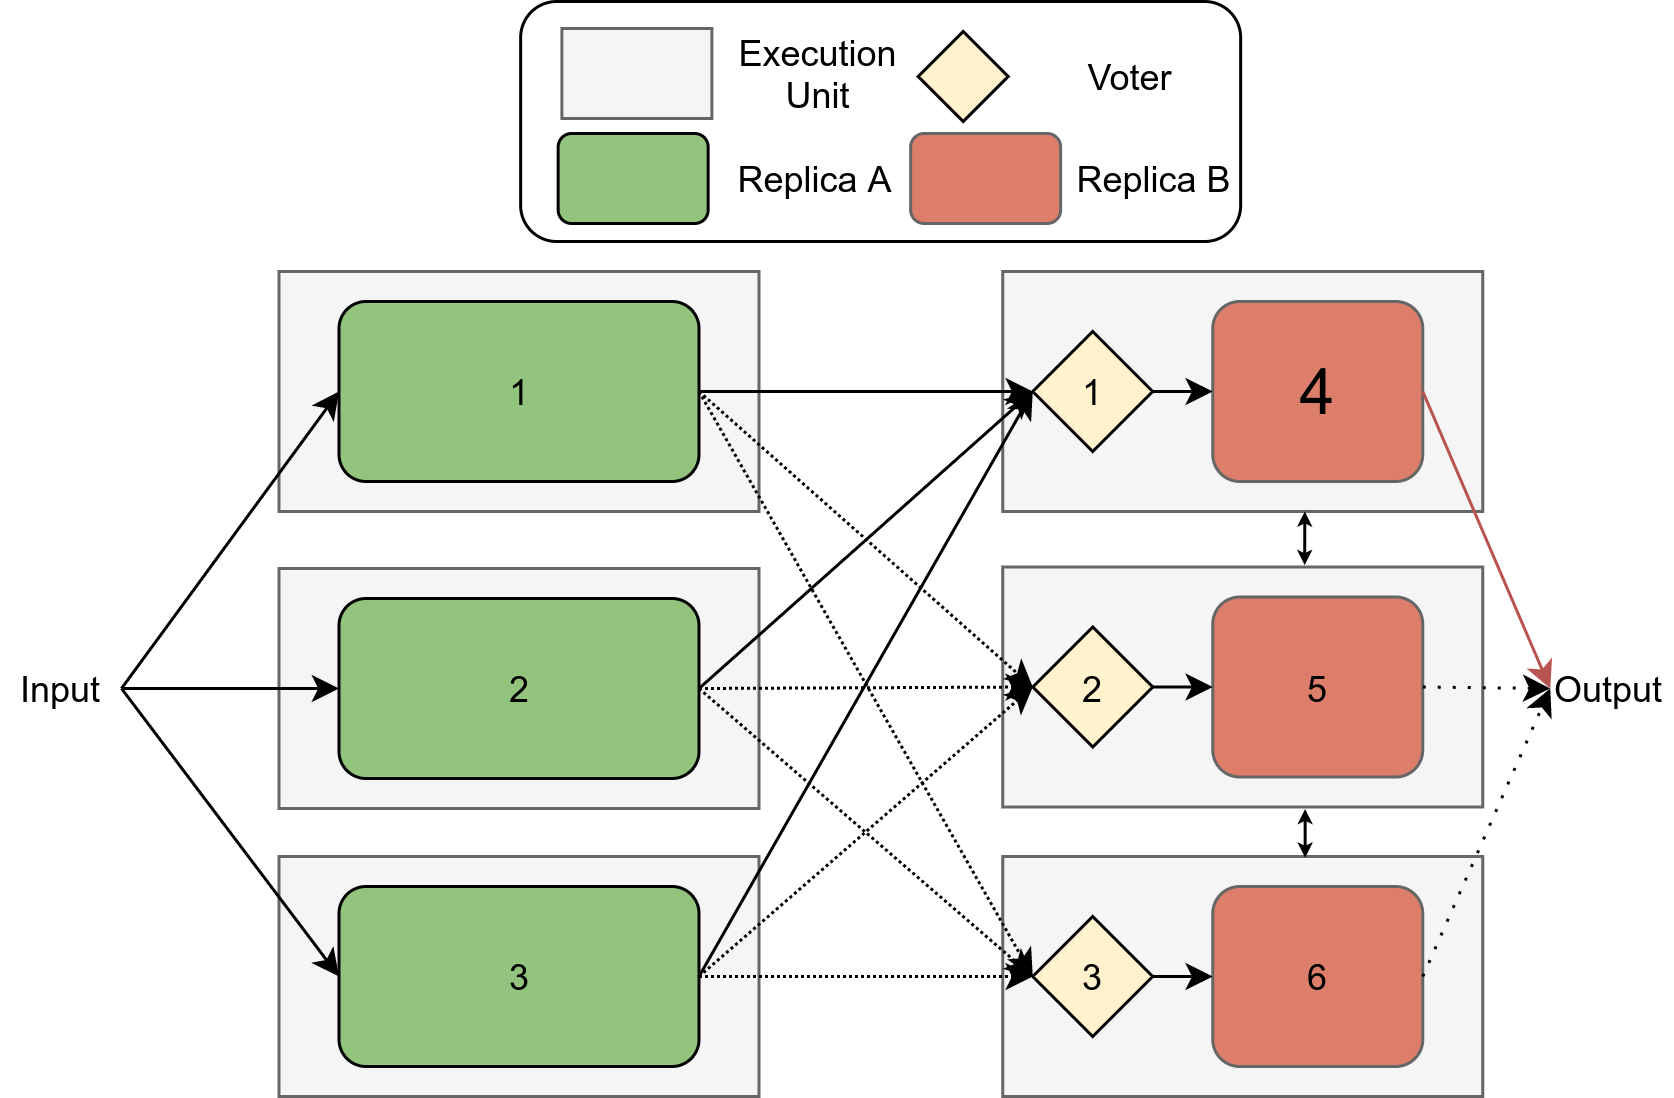
\includegraphics[width=0.8\linewidth]{images/ThreeComponentConsensus}
	\caption{In a consensus-based architecture, no component is a single point of failure. Instead, the components agree on how the output is generated. In this example, voter \textbf{(4)} performs a majority voting on the redundant results from the replicas of type \textbf{A}. Type \textbf{B} replicas implement the consensus algorithm and agree on who controls the output.}
	\label{fig:ThreeRepConsensus}
\end{figure}

For a consensus, multiple components are involved in deciding about redundant information.
An exemplary consensus algorithm is \texttt{Raft}, which has been proposed by Ongaro and Ousterhout~\cite{RaftConsensusPaper}.
A component in \texttt{Raft} can take on one of three roles, namely \textit{leader}, \textit{follower}, or \textit{candidate}.
While a leader takes over the entire responsibility in the system, followers wait for instructions from the leader.
Followers can become candidates to run for the new leader.
\texttt{Raft}'s leader election algorithm ensures that only one leader is active at a time and that the absence of a leader in the system is reliably detected.

An example of how the three roles from \texttt{Raft} are used is depicted in~\autoref{fig:ThreeRepConsensus}.
The replicas \textbf{(1)}, \textbf{(2)}, and \textbf{(3)} make up a \abr{TMR} system, while replicas \textbf{(4)}, \textbf{(5)}, and \textbf{(6)} together define a voter for the system.
The replicas \textbf{(4)}, \textbf{(5)}, and \textbf{(6)} together implement the consensus protocol and each provides a designated voter.
In the example of~\autoref{fig:ThreeRepConsensus}, replica (4) took over the leader role and thereby had complete control over the output, while \textbf{(5)} and \textbf{(6)} are followers.
\\

\noindent
A consensus-inspired redundant application provides a way to address the \ChallengeVoter problem.
In \texttt{Raft}, this is done via periodic heartbeat message that is sent by the voter.
If the voter crashes, the messages stay out and a new voter can be elected.
However, a consensus-based architecture increases the system's communication overhead and can introduce new problems such as split brains.


\section{System Decision}
In this chapter, starting from \abr{TMR}, different redundant architectures were analyzed and evaluated in terms of reliability, security, and feasibility with \abr{DDS}.
In \abr{TMR}, three challenges affected the system's safety.
The problem of \ChallengeWR was addressed by adding additional replicas, e.g. via active hardware redundancy.
In order to overcome the \ChallengeThrough and increase the system's throughput, a pipelined approach was introduced.
Finally, a consensus-inspired architecture was introduced to meet the challenge of \ChallengeVoter.
\\

\noindent
Throughout this section, a final decision regarding a redundant architecture will be made.
This architecture is implemented to show its feasibility with the \abr{DCPS} communication model and its consistency with the fault model.
The implementation is described in~\autoref{cpt:Implementation}.

\subsection{System Architecture}
\label{subsec:SystemArchitecture}

The redundant architecture, which meets all the requirements in terms of reliability and safety, is a combination of the architectures described above and depicted in~\autoref{fig:ThreeRepConsensusDDS}.
The basic architecture is similar to a pipelined \abr{TMR} with a spare and an elected voter.
On the one hand, an input processing unit is responsible for reading inputs, making decisions, and communicating the decisions to the consensus component.
On the other hand, a consensus component implements the leader election logic, exchanges votes with other replicas, requests decisions from input processing units, performs votes on decisions, and controls the system's output.
Further, a spare unit is used that can be activated or deactivated by the system's leader.
\texttt{Raft} lays the foundation for the applied consensus algorithm.

\begin{figure}[!ht]
	\centering
	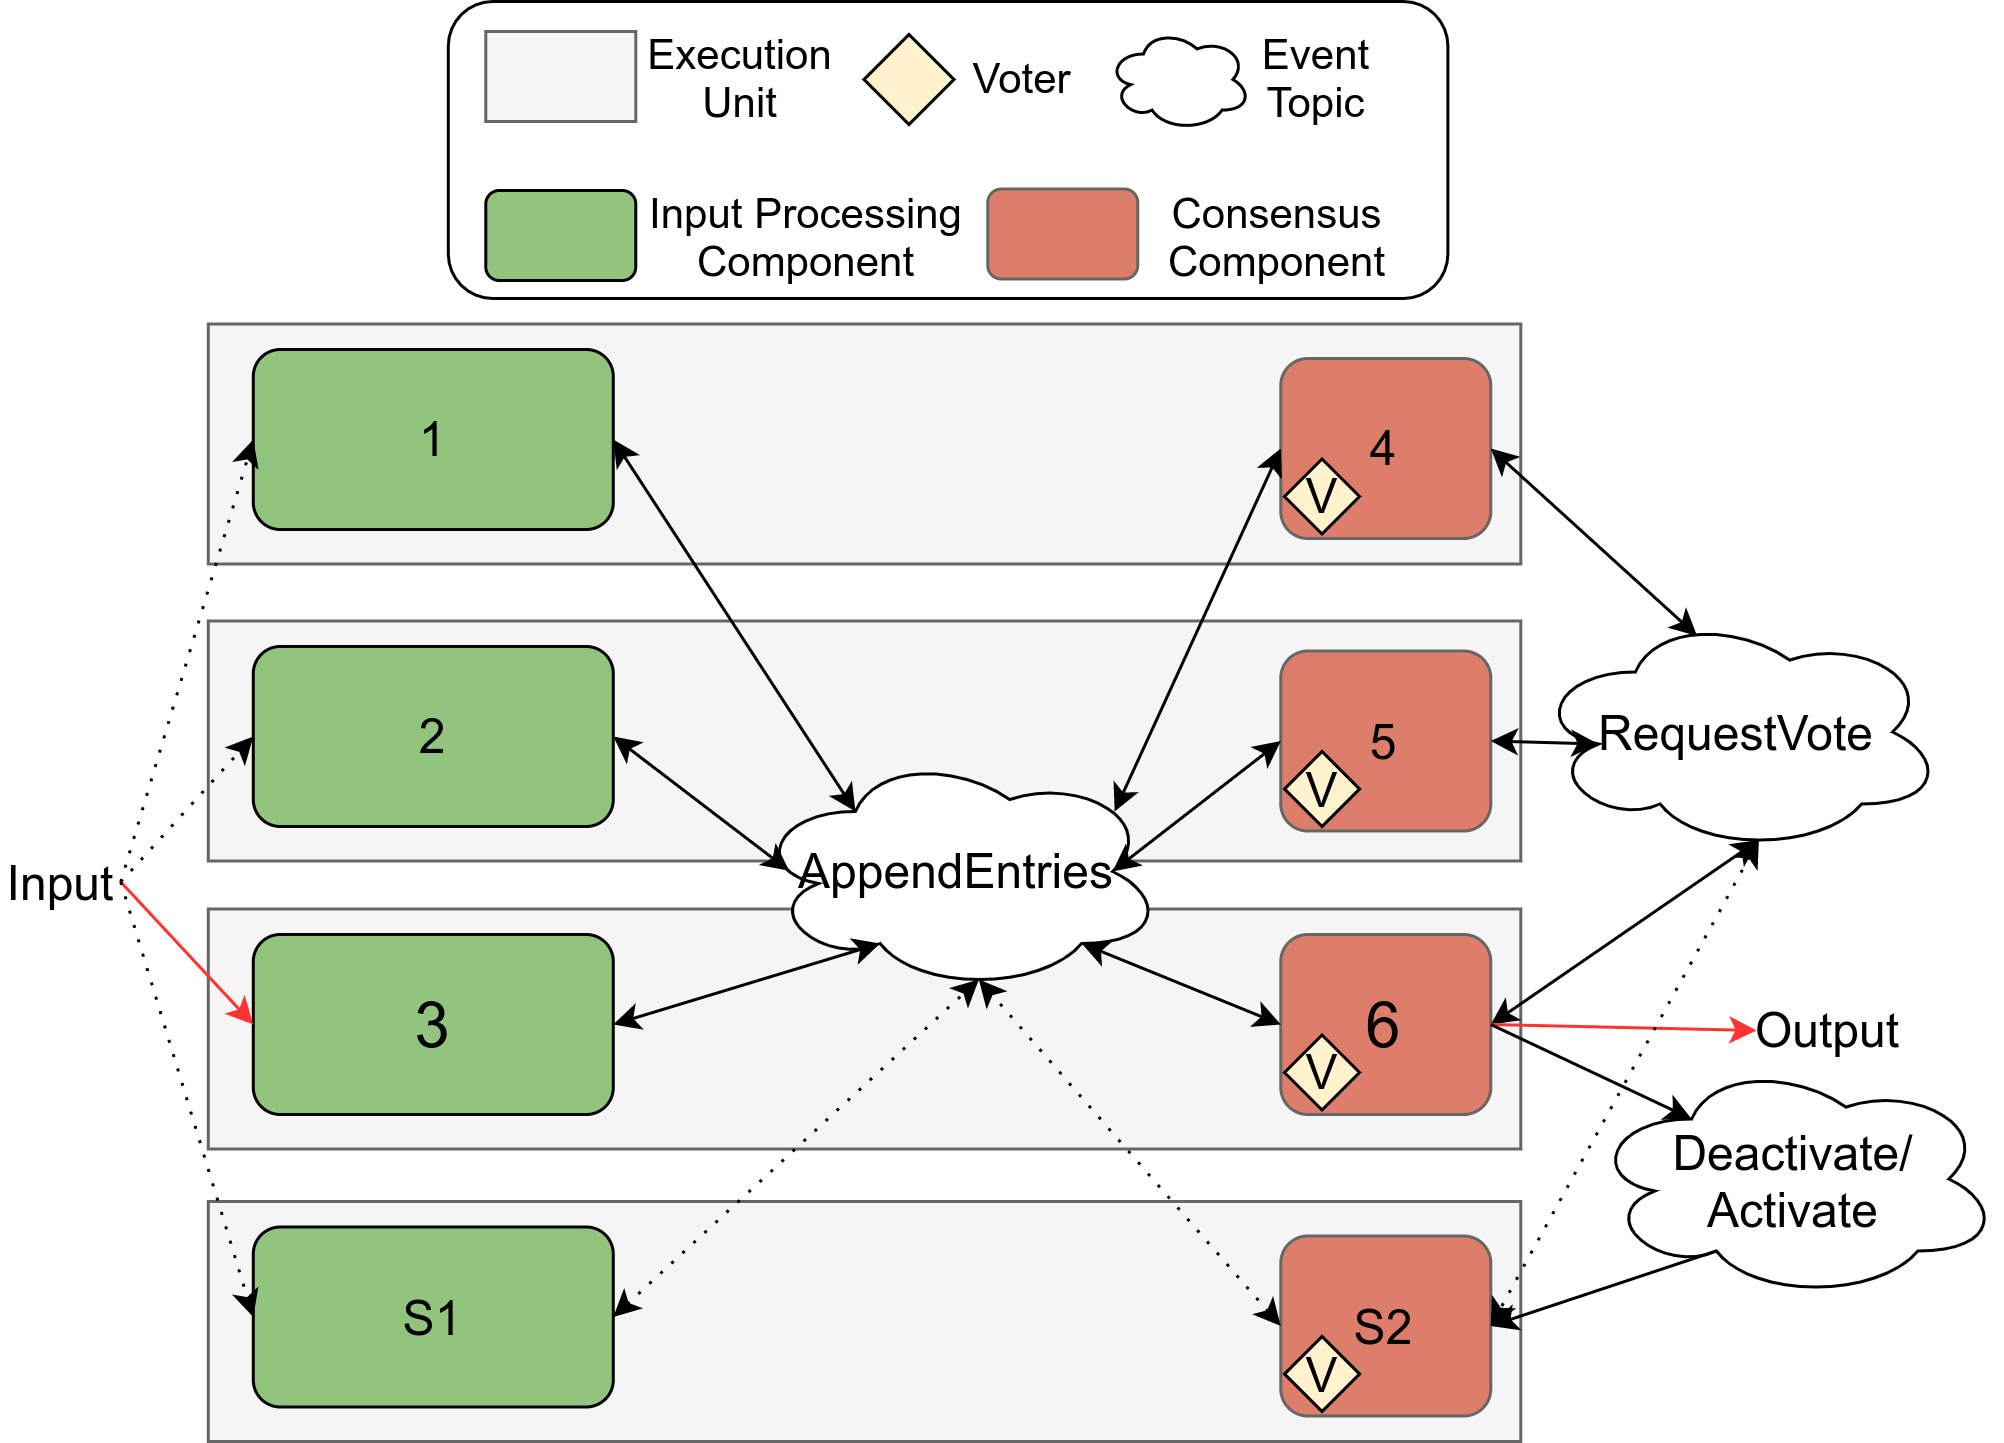
\includegraphics[width=0.9\linewidth]{images/ThreeEUConsensusDDS}
	\caption{An approach for building a hybrid consensus- and voting-based \abr{TMR} system using \abr{DDS} event topics. The approach follows concepts of \texttt{Raft}. In \texttt{Raft}, replicas communicate via \abrpl{RPC}. At least two \abrpl{RPC} are required, namely \texttt{RequestVote} and \texttt{AppendEntries}. \texttt{RequestVote} is used for electing a system leader and is accessed by the consensus component. \texttt{AppendEntries} is used to send heartbeat messages and exchange logs, such as inputs and decisions, between the input processing and the consensus component. The consensus component has an integrated voter for voting on decisions. In this example, \abr{EU} with \textbf{(3)} and \textbf{(6)} took over the leader role and thereby reads inputs and controls the output.}
	\label{fig:ThreeRepConsensusDDS}
\end{figure}

\noindent
In \texttt{Raft}, it is the leader's responsibility to send periodic heartbeat messages to notify followers about its existence.
The heartbeat messages, as well as all other messages in \texttt{Raft}, are expressed as \abrpl{RPC}.
At least two \abrpl{RPC} need to be supported, namely \texttt{AppendEntries} and \texttt{RequestVote}.
\texttt{AppendEntries} is used for sending heartbeat messages and other commands - called logs in \texttt{Raft} - while \texttt{RequestVote} is invoked by candidates to gather votes to become the new leader.
Since \abr{DDS} will be used for communication, the \abrpl{RPC}, as well as the \texttt{Deactivate/Activate} topic, are represented by \abr{DDS} event topics.
\\

\noindent
In the example depicted in~\autoref{fig:ThreeRepConsensusDDS}, the \abr{EU} with input processing component \textbf{(3)} and consensus component \textbf{(6)} took over the leader role.
Hence, \textbf{(3)} reads the input data and requests a decision from \textbf{(1)} and \textbf{(2)} via the \texttt{AppendEntries} topic.
After \textbf{(1)} and \textbf{(2)} have published their decision, \textbf{(6)} can perform the voting and output the voted result.
\\

\noindent
\texttt{AppendEntries} is further used for heartbeat messages.
When a heartbeat message stays out for a period, the remaining replicas assume that the leader has crashed and the followers initiate a new leader election using the \texttt{RequestVote} topic.
When a new leader is elected, it gains complete control over the output, reads input data, and starts sending heartbeat messages.
In the event of the previous leader coming back online again, it receives heartbeat messages from \texttt{AppendEntries} and hence takes over a follower role.
Thereby, crash faults (\textbf{F1}) for voters can be caught by the heartbeat mechanism.

Nevertheless, it is not possible to catch omission, timing, and computation faults for voters with the considered consensus-inspired architecture.
This is because the voter, which acts as the system's leader, has sole responsibility and control over the system's output.
When the voter fails to perform voting on incoming decisions, the system's output remains unchanged and thus the system's safety is affected.
However, a majority voting algorithm is quite simple and the applied fault model presupposes the correct transmission of data. Thus, omission, timing, and computation faults are unlikely to happen for the voter.
Further, additional hardware could be applied to catch omission and timing faults for voters.
For example, a hardware timer could be started as soon as input data is recognized and stopped when the system produced an output.
When the hardware timer is not stopped after a timeout is expired, the train can be stopped.
\\

\noindent
Even though the approach presented in~\autoref{fig:ThreeRepConsensusDDS} resembles a pipelined approach, each pipeline is executed on the same \abr{EU}.
In order to benefit from throughput benefits, each pipeline step should be placed on a different \abr{EU}, though.
Nevertheless, the presented approach does not suffer from a \ChallengeThrough so that a single \abr{EU} for each pipeline is sufficient.
Further, the approach allows for more replicas by distributing the logic modules accordingly.
This is because the components communicate via \abr{DDS} topics and are thereby freely scalable.

\subsection{Communication Model}
All computing systems have in common that they receive an input and produce an output.
In the exemplary case that is considered in this thesis, inputs consist of \abrpl{MA}, balise linking information, and balise telegrams.
The inputs are expected to be transmitted via an \texttt{Input} \abr{DDS} topic.
Such an \texttt{Input} topic should be defined as an event topic to make sure that every replica receives and eventually processes the inputs.
Because inputs occur asynchronously, the deadline \gls*{QOS} is not applicable for the \texttt{Input} event topic.
For the real-time application examined in this work, an output is expected to be delivered by the system within a maximal timespan of $\Delta t$ after the system received an input.
Therefore, the input topic's \texttt{Durability} should be set to volatile and the \texttt{Lifespan}-policy can be set to at least $\Delta t$ plus a network latency.
There are also other ways for ensuring deadlines in \abr{DDS}, such as using \texttt{WaitSets} that can be attached with timeouts.
As mentioned by Sinha \etal, network latency can be measured with a looping technique that utilizes \abr{IP} \abr{TTL} or by an end-to-end approach using probing packets~\cite{SinhaMeasureNetworkLatency}.
Latter is applied in~\autoref{cpt:evaluation} to determine network characteristics in the practical approach.
The input's \texttt{ResourceLimit} depends on the frequency the input is expected to be delivered and can be set to one when the input's frequency is higher than $\Delta t$.
\\

\noindent
The components in a redundant system are required to communicate with one another because at the end, the entire system needs to present a single result.
In the course of this thesis, all communication in the system will be implemented using \abr{DDS} event topics because it should be ensured that, given a sufficient network, no information is lost in the system.
Thus, the communication topic's \gls*{QOS}-settings can be the same as for the input topic.
However, the \texttt{Lifespan}-policy and timeouts require further specification because the replicas are independent and messages might be delayed due to network latency.
After a specific time, however, a certain message might not be valid anymore.
An example of this could be a message concerning a \abr{MA} that has been expired by the time the delayed information was received.
Hence, a component's message might require a certain \texttt{Lifespan}-policy or timeout that depends on the actual message.
\\

\noindent
So that all replicas can make deterministic decisions in specific situations, they must have access to a global system state.
Such a global system state should store the currently valid \abr{MA}, a set of linked balises, as well as the train's current speed and estimated position.
Since \abr{MA} and balise linking information is communicated at the start of each journey, they are each stored in an enduring \abr{DDS} state topic.
The train's state is expected to change frequently, so that it is stored in a volatile \abr{DDS} state topic.